\documentclass[english,10pt,a4paper]{article}
\usepackage{tcolorbox}
\usepackage{ulem} %math
\usepackage{amsmath}
\usepackage{amsfonts}
\usepackage{amssymb}
\usepackage{graphicx}
\usepackage{enumerate}


%Create a box for theorems
%\begin{theo}[titel] %optional
%tekst
%\end{theo}
\newenvironment{theo}[1][Vigtigt]{%
\begin{tcolorbox}[colback=green!5,colframe=green!40!black,title=\textbf{#1}]
}{%
\end{tcolorbox}
}




%Create a square matrix
%\begin{ArgMat}{2}
%21 & 22 & 23 \\  
%a & b & c
%\end{ArgMat}
%
% Info: http://tex.stackexchange.com/questions/2233/whats-the-best-way-make-an-augmented-coefficient-matrix
%
\newenvironment{ArgMat}{%
$
  \left[\begin{array}{@{}*{100}{r}r@{}}
}{%
  \end{array}\right]
  $
}

\newenvironment{deter}{%
$
  \left|\begin{array}{@{}*{100}{r}r@{}}
}{%
  \end{array}\right|
  $
}


%Create multiple lines with holes
%\begin{SysEqu}
%x_1 && &- &5x_3 &+ &2x_4=& 1 \\
%x_1 &+ &x_2 &+ &x_3 && =& 4 \\
%&&&&&&0 =& 0
%\end{SysEqu}
\newenvironment{SysEqu}{%
$  \setlength\arraycolsep{0.1em}
  \begin{array}{@{}*{100}{r}r@{}}
}{%
  \end{array}$
}

%Create solution for x_1, x_n...
%\begin{solu}
%x_1 &= d \\
%x_2 &= e \\
%x_3 &= s
%\end{solu}
\newenvironment{solu}{%
$
  \setlength\arraycolsep{0.1em}
  \left\{\begin{array}{@{}*{100}{r}r@{}}
}{%
  \end{array}\right.
$
}

\usepackage{lastpage}


\newcommand{\HRule}{\rule{\linewidth}{0.8mm}}

%Tekst i fotter
\newcommand{\footerText}{\thepage\xspace /\pageref{LastPage}}
\newcommand{\ProjectName}{433 MHz styring af AeroQuad}


\chapterstyle{hangnum}




\nouppercaseheads
\makepagestyle{mystyle} 

\makeevenhead{mystyle}{}{\\ \leftmark}{} 
\makeoddhead{mystyle}{}{\\ \leftmark}{} 
\makeevenfoot{mystyle}{}{\footerText}{} 
\makeoddfoot{mystyle}{}{\footerText}{} 
\makeatletter
\makepsmarks{mystyle}{% Overskriften på sidehovedet
  \createmark{chapter}{left}{shownumber}{\@chapapp\ }{.\ }} 
\makeatother
\makefootrule{mystyle}{\textwidth}{\normalrulethickness}{0.4pt}
\makeheadrule{mystyle}{\textwidth}{\normalrulethickness}

\makepagestyle{plain}
\makeevenhead{plain}{}{}{}
\makeoddhead{plain}{}{}{}
\makeevenfoot{plain}{}{\footerText}{}
\makeoddfoot{plain}{}{\footerText}{}
\makefootrule{plain}{\textwidth}{\normalrulethickness}{0.4pt}

\pagestyle{mystyle}

%%----------------------------------------------------------------------
%
%%Redefining chapter style
%%\renewcommand\chapterheadstart{\vspace*{\beforechapskip}}
%\renewcommand\chapterheadstart{\vspace*{10pt}}
%\renewcommand\printchaptername{\chapnamefont }%\@chapapp}
%\renewcommand\chapternamenum{\space}
%\renewcommand\printchapternum{\chapnumfont \thechapter}
%\renewcommand\afterchapternum{\space: }%\par\nobreak\vskip \midchapskip}
%\renewcommand\printchapternonum{}
%\renewcommand\printchaptertitle[1]{\chaptitlefont #1}
\setlength{\beforechapskip}{0pt} 
\setlength{\afterchapskip}{0pt} 
%\setlength{\voffset}{0pt} 
\setlength{\headsep}{25pt}
%\setlength{\topmargin}{35pt}
%%\setlength{\headheight}{102pt}
%\setlength{\textheight}{302pt}
\renewcommand\afterchaptertitle{\par\nobreak\vskip \afterchapskip}
%%----------------------------------------------------------------------




%Sidehoved og -fod pakke
%Margin
\usepackage[left=2cm,right=2cm,top=2.5cm,bottom=2cm]{geometry}
\usepackage{lastpage}



%%URL kommandoer og sidetal farve
%%Kaldes med \url{www...}
%\usepackage{color} %Skal også bruges
\usepackage{hyperref}
\hypersetup{ 
	colorlinks	= true, 	% false: boxed links; true: colored links
    urlcolor	= blue,		% color of external links
    linkcolor	= black, 	% color of page numbers
    citecolor	= blue,
}



%Mellemrum mellem linjerne    
\linespread{1.5}


%Seperated files
%--------------------------------------------------
%Opret filer således:
%\documentclass[Navn-på-hovedfil]{subfiles}
%\begin{document}
% Indmad
%\end{document}
%
% I hovedfil inkluderes således:
% \subfile{navn-på-subfil}
%--------------------------------------------------
\usepackage{subfiles}

%Prevent wierd placement of figures
%\usepackage[section]{placeins}

%Standard sti at søge efter billeder
%--------------------------------------------------
%\begin{figure}[hbtp]
%\centering
%\includegraphics[scale=1]{filnavn-for-png}
%\caption{Titel}
%\label{fig:referenceNavn}
%\end{figure}
%--------------------------------------------------
\usepackage{graphicx}
\usepackage{subcaption}
\usepackage{float}
\graphicspath{{../Figures/}}

%Speciel skrift for enkelt linje kode
%--------------------------------------------------
%Udskriver med fonten 'Courier'
%Mere info her: http://tex.stackexchange.com/questions/25249/how-do-i-use-a-particular-font-for-a-small-section-of-text-in-my-document
%Eksempel: Funktionen \code{void Hello()} giver et output
%--------------------------------------------------
\newcommand{\code}[1]{{\fontfamily{pcr}\selectfont #1}}


% Følgende er til koder.
%----------------------------------------------------------
%\begin{lstlisting}[caption=Overskrift på boks, style=Code-C++, label=lst:referenceLabel]
%public void hello(){}
%\end{lstlisting}
%----------------------------------------------------------

%Exstra space
\usepackage{xspace}
%Navn på bokse efterfulgt af \xspace (hvis det skal være mellemrum
%gives det med denne udvidelse. Ellers ingen mellemrum.
\newcommand{\codeTitle}{Kodeudsnit\xspace}

%Pakker der skal bruges til lstlisting
\usepackage{listings}
\usepackage{color}
\usepackage{textcomp}
\definecolor{listinggray}{gray}{0.9}
\definecolor{lbcolor}{rgb}{0.9,0.9,0.9}
\renewcommand{\lstlistingname}{\codeTitle}
\lstdefinestyle{Code}
{
	keywordstyle	= \bfseries\ttfamily\color[rgb]{0,0,1},
	identifierstyle	= \ttfamily,
	commentstyle	= \color[rgb]{0.133,0.545,0.133},
	stringstyle		= \ttfamily\color[rgb]{0.627,0.126,0.941},
	showstringspaces= false,
	basicstyle		= \small,
	numberstyle		= \footnotesize,
%	numbers			= left, % Tal? Udkommenter hvis ikke
	stepnumber		= 2,
	numbersep		= 6pt,
	tabsize			= 2,
	breaklines		= true,
	prebreak 		= \raisebox{0ex}[0ex][0ex]{\ensuremath{\hookleftarrow}},
	breakatwhitespace= false,
%	aboveskip		= {1.5\baselineskip},
  	columns			= fixed,
  	upquote			= true,
  	extendedchars	= true,
 	backgroundcolor = \color{lbcolor},
	lineskip		= 1pt,
%	xleftmargin		= 17pt,
%	framexleftmargin= 17pt,
	framexrightmargin	= 0pt, %6pt
%	framexbottommargin	= 4pt,
}

%Bredde der bruges til indryk
%Den skal være 6 pt mindre
\usepackage{calc}
\newlength{\mywidth}
\setlength{\mywidth}{\textwidth-6pt}


% Forskellige styles for forskellige kodetyper
\usepackage{caption}
\DeclareCaptionFont{white}{\color{white}}
\DeclareCaptionFormat{listing}%
{\colorbox[cmyk]{0.43, 0.35, 0.35,0.35}{\parbox{\mywidth}{\hspace{5pt}#1#2#3}}}
\captionsetup[lstlisting]
{
	format			= listing,
	labelfont		= white,
	textfont		= white, 
	singlelinecheck	= false, 
	width			= \mywidth,
	margin			= 0pt, 
	font			= {bf,footnotesize}
}

\lstdefinestyle{Code-C} {language=C, style=Code}
\lstdefinestyle{Code-Java} {language=Java, style=Code}
\lstdefinestyle{Code-C++} {language=[Visual]C++, style=Code}
\lstdefinestyle{Code-VHDL} {language=VHDL, style=Code}
\lstdefinestyle{Code-Bash} {language=Bash, style=Code}

%Text typesetting
%--------------------------------------------------------
%\usepackage{baskervald}
\usepackage{lmodern}
\usepackage[T1]{fontenc}              
\usepackage[utf8]{inputenc}         
\usepackage[english]{babel}       

\setlength{\parindent}{0pt}
\nonzeroparskip

%\setaftersubsecskip{1sp}
%\setaftersubsubsecskip{1sp}
 


%Dybde på indholdsfortegnelse
%----------------------------------------------------------
%Chapter, section, subsection, subsubsection
%----------------------------------------------------------
\setcounter{secnumdepth}{3}
\setcounter{tocdepth}{3}


%Tables
%----------------------------------------------------------
\usepackage{tabularx}
\usepackage{array}
\usepackage{multirow} 
\usepackage{multicol} 
\usepackage{booktabs}
\usepackage{wrapfig}
\renewcommand{\arraystretch}{1.5}



%Misc
%----------------------------------------------------------
\usepackage{cite}
\usepackage{appendix}
\usepackage{amssymb}
\usepackage{url,ragged2e}
\usepackage{enumerate}
\usepackage{amsmath} %Math bibliotek


\usepackage{longtable}


\title{Handin 2}
\author{10893, Rasmus Bækgaard}
\date{September 6th, 2013}
\begin{document}
\maketitle

\section*{Problem 1}
Let \textit{S} denote the set of odd integers and let $P(x): x2 + 1$ is even and $Q(x): x2$ is even be open sentences over \textit{S}. 
State $\forall x \in S, P(x)$ and $\exists x \in S, Q(x)$ in words. 
What is the truth value?
\\
\\
$P(x)$: For all elements in \textit{S}, $P(x) = x^2 +1$. 
This is true, since all odd, square values are odd and plus one give an even number.
\\
$Q(x)$: For some elements in \textit{S}, $Q(x)=x^2$. This is false, since odd, square values are odd.


\section*{Problem 2}
Let $P(n): \dfrac{5n-6}{3}$ is an integer be an open sentence over the domain $\mathbb{Z}$. Determine, with explanations, whether the following statements are true:
\begin{enumerate}[a]
\item $\forall z \in \mathbb{Z}, P(z)$
\item[] This statement is false, since not all integer values will give an integer. 
Example: $\dfrac{5\cdot 1-6}{3}=\dfrac{-1}{3} \not = \mathbb{Z}$
\item $\exists z \in \mathbb{Z}, P(z)$
\item[] This statement is true, since some integer values will give an integer. 
Example: $\dfrac{5\cdot 6 - 6}{3}=\dfrac{24}{3} = 8  = \mathbb{Z}$
\end{enumerate}



\section*{Problem 3}
It is tempting to think that, if a statement involving the natural number \textit{n} is true for many consecutive values of \textit{n}, it must be true for all \textit{n}. 
In that connection the example from Euler is illustrative.
 Let $f(n) = n^2 + n + 41$ 
\begin{enumerate}[a]

\item Convince yourself (perhaps with the use of Mable or another tool) that f(1), f(2), … f(39) is prime, but f(40) is not. 
\item[] Write a script in \textbf{MatLab} as follow:
\end{enumerate}

\begin{lstlisting}[caption=title, style=Code-Matlab, label=lst:ref]
syms n;
f(n) =n^2+n+41;
ArrSize = 40;
Array=[zeros(ArrSize,3)];

for i=1: ArrSize
    Array(i,1) = i;
    Array(i,2) =f(i);
    Array(i,3) = isprime(Array(i,2));
end
Array
\end{lstlisting}
\begin{enumerate}[b]
\item[] Looking at the array list will show the values and if it's a prime number or not ( mark with '1' for \textit{true} and '0' for \textit{false}).
Since the array list does not contain a '0' they are all primes but the last element.

\item Show that, for any \textit{n} of the form $n = k^2 + 40$, \textit{f(n)} is not prime.
\item[] If $f(n)$ is not a prime, it means atleast 2 values can be added to each other and it will give $f(n)$.
\begin{align}
\text{If } n &= k^2 + 40 \\
f(n) &=\Big(k^2+40\Big)^2+\Big(k^2+40\Big)+41  & \text{Insert \textit{n} in } f(n)\\
f(k) &= k^4 + 40^2 +80k^2+ k^2+40+41 & \text{Dissolve the paratheses}\\
	&= k^4+81k^2+1681 & \text{Sum up}\\
	&= k\bigg(k^3 + 81k+\dfrac{1681}{k}\bigg) &k \text{ outside paratheses}\\
	&= k \cdot x & \text{Notice it is a product} \label{equ:product}
\end{align}
\item[] From (\ref{equ:product}) we can see, that $f(n)$ is not a prime, since any number, \textit{k}, inserted in $f(k) =\Big(k^2+3k+41 \Big)^2$ gives a non-prime which means for any value we assign \textit{k} in $n=k^2+40$ will give us a non-prime.
\end{enumerate}



\section*{Problem 4}
Prove that between any two different rational numbers there is another rational number.
\\
\\
Since a rational number is a number expressed by two numbers, like $\dfrac{m}{n}$ you can always find a number between two other rational numbers.
This is due to the amount of decimal will increase with higher numbers and if the rational numbers goes to rational you can always find a number between two rational numbers.


\section*{Problem 5}
Let $n \in N$. Prove that if $n^3 - 5n - 8 > 0$ then $n \geq 3$. What proof technique did you use? Why?
\\
\\
An easy illustration, Figure \ref{fig:prob5}, created in \textbf{Matlab} will show why only the natural numbers from 3 and above is positive:

\begin{lstlisting}[caption=title, style=Code-Matlab, label=lst:ref]
n=0.1:1:10;
f=power(n,3)-5*n-8;
figure(1)
subplot(1,1,1)
plot(n, f, 's', n, f)
axis([0 5 -25 100])
title('f(n)')
set(gca, 'XTick', [0:1:6])
set(gca, 'YTick', [0])
grid on
\end{lstlisting}
\begin{figure}[hbtp]
\centering
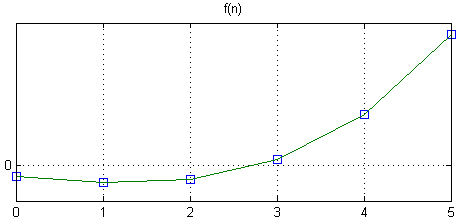
\includegraphics[scale=0.9]{H2-5}
\caption{Diagram of equation}
\label{fig:prob5}
\end{figure}

Also the equation can be rewritten as follow:
\begin{align}
n^3-5n-8 &> 0 &\\
n^3-5n &> 8 & & \text{Move the }8\\
n(n^2-5) &> 8 & & \text{Isolate \textit{n} on left side} \label{equ:iso}
\end{align}

Looking at (\ref{equ:iso}) it shows that $n^2-k$ is only getting bigger and bigger and with the scale outside it will always increase in value, as soon as it is positive, like $n=3 \Rightarrow 3^2-5 = 9-5=4$ but not $n=2 \Rightarrow 2^2-5=4-5=-1$.
\\
\\
However it is perhaps clearer to see if we make it contrapositive:\\
Prove that if $n^3 - 5n - 8 < 0$ then $n < 3$\\
\\
Now only the values 0, 1 and 2 must be calculated:
\begin{align*}
0^3-5 \cdot 0 - 8 &= -8 & True\\
1^3-5\cdot 1-8 &= -12 & True\\
2^3-5\cdot 2-8 &= -10 & True\\
3^3-5\cdot 3-8 &= 5 & False
\end{align*}
The methods used are contrapositive proof, simple figures and logic explaining the coherence of the numbers, along with isolated examples.
\\
The contrapositive method is good for showing a few numbers,
The figure is good to use since figure tells more faster than plain numbers.


\section*{Problem 6}
Prove that $\overline{A \cap B} = \overline{A} \cup \overline{B}$ for every two sets \textit{A} and \textit{B}. Does it hold for the empty set as well?
\\
\\
To prove the statement we'll use DeMorgan's II law:
\begin{align}
\overline{A \cap B} &= \overline{(\overline{\overline{A}} \cap \overline{\overline{B}})} & \text{Double negation}\\
	&= \overline{\overline{(\overline{A} \cup \overline{B})}} & \text{DeMorgan's I law}\\
	&= \overline{A} \cup \overline{B} & \text{Double negation} 
\end{align}

It can hold empty sets -- The inverse of $\emptyset$ is everything. 
And the union of everything and everything is it all.


\section*{Problem 7}
Let \textit{A, B} and \textit{C} be sets. Prove that $\overline{\overline{A} \cup \big( \overline{B} \cap C \big)} = (A \cap B) \cup (A - C)$:

\begin{align}
\overline{\overline{A} \cup \big( \overline{B} \cap C \big)} 
	&= A \cap ( B \cup \overline{C}) & \text{DeMorgan's II law}\\
	&= (A \cap B) \cup (A \cap \overline{C}) & \text{Associative law} \\
	&= (A \cap B) \cup (A - C) &
\end{align}



\section*{Problem 8}
Let \textit{A, B} and \textit{C} be sets. Prove that $(A-B) \cap (A-C) = A-(B\cup C)$:

\begin{align}
(A-B) \cap (A-C) &=(A \cap \overline{B}) \cap (A \cap \overline{C})\\
	&=(A \cap A)  \cap (\overline{B} \cap \overline{C}) & \text{Assosiative law}\\
	&= A \cap (\overline{B} \cap \overline{C})\\
	&= A \cap (\overline{B \cup C}) & \text{DeMorgan}\\
	&= A-(B\cup C) & \text{See problem 7 or the book p. 109}
\end{align}




\section*{Problem 9}
What is wrong with the following “proof”? 
Let $a, b \in \mathbb{R}$ and $a=b$.

\begin{align}
a &=b &  Good\\
ab&=b^2 & Good\\
ab-a^2 &= b^2-a^2 &Good \\
a(b-a) &= (b-a)(b+1) & \text{Sure thing}\\
a &= b+a & \text{No, }b-a\text{ is }a-a = 0. \text{ Don't divide by 0}
\end{align}


\end{document}